\documentclass[letterpaper, 11pt]{article}
\usepackage{comment} % enables the use of multi-line comments (\ifx \fi) 
\usepackage{fullpage} % changes the margin
\usepackage{fancyhdr} % for footer
\usepackage[UKenglish]{isodate}% http://ctan.org/pkg/isodate for date format
\usepackage[]{natbib}
\usepackage{hyperref}
\usepackage{graphicx}
\usepackage{wrapfig}
\usepackage[font={small,sf}]{caption}

\pagestyle{fancy}
\renewcommand{\headrulewidth}{0pt}

\lhead{}
\chead{}
\rhead{}
\lfoot{ENT 432 (Fall 2016) - Penn State}
\cfoot{}
\rfoot{\thepage}
\renewcommand{\footrulewidth}{0.4pt}
\title{Discover your inner Darwin}% need sexier title
\author{Open Entomology Project}

\begin{document}
\cleanlookdateon %removed ordinal date
\maketitle
\thispagestyle{fancy}

\section*{Background}
\begin{wrapfigure}{r}{0.5\textwidth}
  \vspace{-20pt}
  \begin{center}
    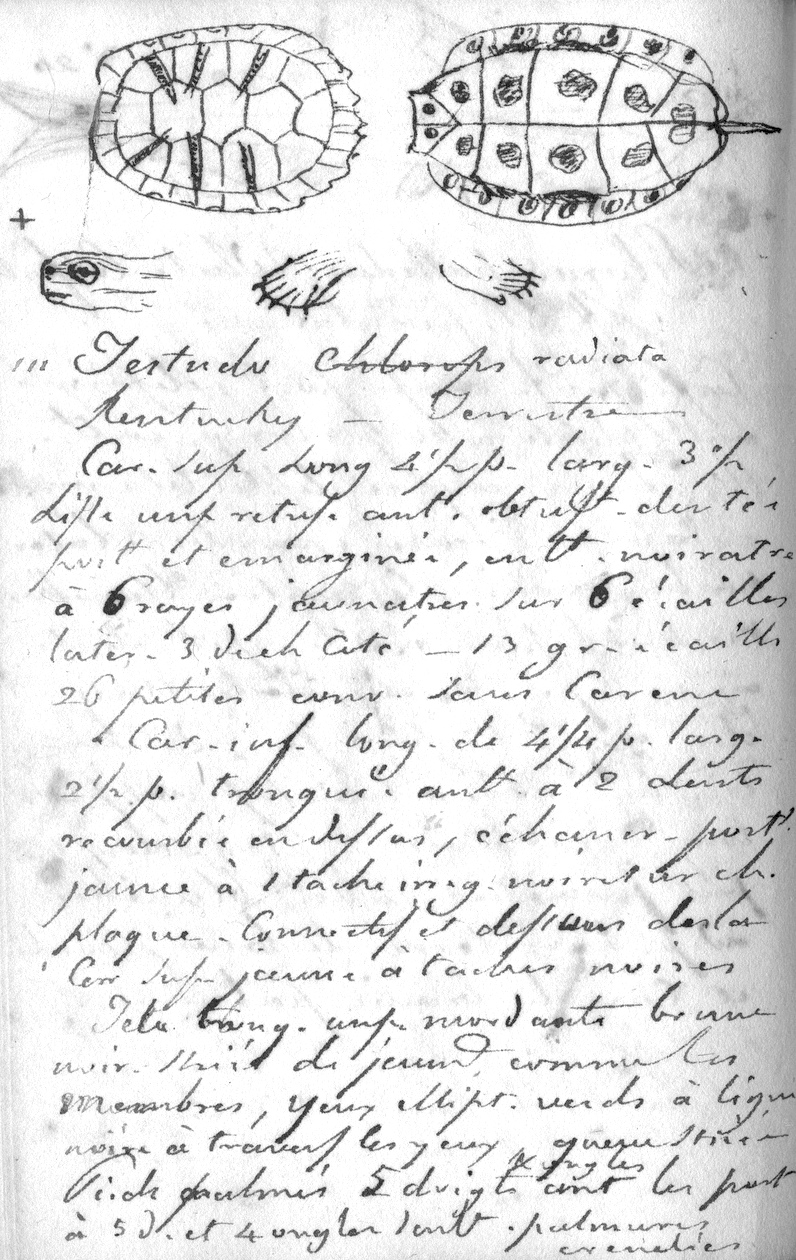
\includegraphics[width=0.38\textwidth]{Rafinesque}
  \end{center}
  \vspace{-16pt}
  \caption{A page from Constantine Rafinesque's (1818) field notebook. What would a page from yours look like? See original image: \url{https://flic.kr/p/dbEePV}}
  \vspace{-38pt}
\end{wrapfigure}
Entomology is informed, enriched, and inspired by a broad knowledge of natural history, what \cite{Tewksbury01042014} refer to as the ``fundamental properties of organisms''. We cover insect natural history extensively in lecture discussions and lab exercises---what insects eat, how they reproduce, how to diagnose taxa, how taxa are related, adaptations they have, how they interact with symbionts, parasites, predators, \textit{etc}. With respect to really understanding and appreciating insects, though, there is no substitute for time spent carefully observing these organisms in their natural environment. 

For this exercise you will spend time---at least 3--4 hours per site---carefully observing and documenting the insect life in two 4 m\textsuperscript{2} areas. You will keep extensive field notes about what you see, and you will collect specimens that serve as vouchers for your observations.

\section*{Your assignment}

\subsection*{Initial Proposal (20 pts.)}
Spend five or ten minutes observing an ant nest, a flower, a spider web, or some other natural object. If you had a pencil and paper what kinds of data would you be recording? What would you sketch? Now imagine that this 5--10 minute exercise was extended into two deep, 4-hour (or longer) sessions, covering two 4 m\textsuperscript{2} in two different habitats. Which habitats would you want to compare? What kinds of supplies and equipment would you need? Note that collecting gear is available through the museum. Other questions to consider in your initial proposal:
\begin{itemize}
\item What are the minimum data you intend to record?
\item How would you collect specimens and label them in a way that they could be associated with the observations you made in your journal? 
\item How would you account for the arthropod fauna you weren't able to observe directly? It's important that you sample your plots extensively, growing your collection beyond those few arthropods you spent time observing.
\item Photos, recordings, and video are not required for these observations. If you do have digital content from these sessions how will you make those available for a broad audience and in a sustainable way?
\end{itemize}

\noindent{}Write your ideas out on a piece of paper, and discuss the approach with your partner. This original proposal should be turned in to your instructors. Don't worry if it's rough around the edges!

\subsection*{Refined Proposal (30 pts.)}
After discussing your approach with your partner(s) did you make any changes? Summarize your conversation and append it to a refined proposal. Make sure this final proposal is logically organized and well-written.

\subsection*{Field Notebook (100 pts.)}
The notebook serves as the record of your natural history observations. It likely will contain substantial data about insects, but it may also include sketches, thoughts, stories, hypotheses, notes about what to do in future observations, \textit{etc}. This component is a substantial portion of your grade for this exercise, and people will have free access to the final product. Any mistakes you make while writing must \textit{NOT} be erased. A single line through the error is sufficient to indicate a mistake.\\

\noindent{}We will provide you with a field notebook that is archival and water resistant (Rite In The Rain No: 371FX, 4 5/8 $\times$ 7$''$, 48 pages). This notebook is property of the Frost Entomological Museum and must be deposited there at the end of the semester. You should use only pencil or an archival ink (\textit{e.g.}, Sakura\textregistered{ }Pigma Micron\textregistered; \url{http://www.pigmamicron.com/museums}); neither of these are provided. 

\subsection*{Field Collection (50 pts.)}
You should collect specimens for each kind of insect you observed, especially if they are the subject of content in your field notebook (\textit{i.e.}, they are vouchers for observations). These specimens must be determined minimally to family, and the collection should be accompanied by a spreadsheet. See the collection guidelines handouts for more details regarding specimen preparation and organization.

\subsection*{Synthesis and highlights (50 pts.)}
During each natural history session there were undoubtedly some insects that you found extraordinarily compelling. They exhibited unusual behavior, for example, or had some unusual phenotype you want to know more about. You should take these specimens, determine them to species, and then research the phenomenon that you found interesting. The results should be summarized in a narrative written for a broad audience---for example, something you would see on a blog---and include references, sketches, photos, \textit{etc}. Alternatively one can develop an oral presentation for the class.

\section*{Further reading}
Numerous authors have highlighted the importance of natural history knowledge for the life sciences. \cite{agrawal2014} and \cite{wilcoveeisner2000} provide relatively simple yet compelling examples of the importance of insect observation. See also \cite{Schmidly449} and \cite{Barrows13042016} for discussions of the importance of natural history as part of the broader life sciences curriculum. For a celebration of field notes, including examples from ecologists, ethologists, systematists, and other scientists see \cite{canfield2011field}. 

% adding bibliography here
\bibliographystyle{apalike}
\bibliography{bib}
\end{document}

Given this paper - http://dx.doi.org/10.1093/biosci/biw043 - perhaps we need a natural history exercise.

(0) Student thinks about his/her background and interests. Based on these and a brief experiment (e.g., watch a spider web for 10 mins) s/he develops a proposed workflow or approach to observing and documenting insect natural history. What materials and supplies will s/he need? How will specimens be matched to observations in a notebook? What kinds of data will be collected? A proposal (1 pg) is written and given to a partner.

(1) Students vet each other's proposal and provide constructive feedback. A refined proposal is turned in for a grade.

(2) Instructors set up 4 m2 areas in different habitats. Students are told which ones they are to spend 4 hours observing/collecting/documenting the insects in it.

(3) Students are then told which one to move to for new observations.

(4) After 2 or 3 iterations student medidates on these observations, discusses them with partner, then chooses 2 or 3 (or 1?) observations s/he wants to develop knowledge on.

(5) The specimens from those key observations get determined to species, there is some literature search, and development of a presentation that is given eventually to the group.

(6) To complement this initial collection, which likely has low diversity relative to all possible insects that occur in PA, students dip into bulk samples taken from similar habitats (e.g., a Malaise trap set up in same meadow for a week). They each need to pull out insects that represent 20 families they didn't observe during their exercise.

(7) The entire collection and raw field notes are turned in, and the stories are presented to the class
